% Options for packages loaded elsewhere
\PassOptionsToPackage{unicode}{hyperref}
\PassOptionsToPackage{hyphens}{url}
%
\documentclass[
]{article}
\usepackage{amsmath,amssymb}
\usepackage{iftex}
\ifPDFTeX
  \usepackage[T1]{fontenc}
  \usepackage[utf8]{inputenc}
  \usepackage{textcomp} % provide euro and other symbols
\else % if luatex or xetex
  \usepackage{unicode-math} % this also loads fontspec
  \defaultfontfeatures{Scale=MatchLowercase}
  \defaultfontfeatures[\rmfamily]{Ligatures=TeX,Scale=1}
\fi
\usepackage{lmodern}
\ifPDFTeX\else
  % xetex/luatex font selection
\fi
% Use upquote if available, for straight quotes in verbatim environments
\IfFileExists{upquote.sty}{\usepackage{upquote}}{}
\IfFileExists{microtype.sty}{% use microtype if available
  \usepackage[]{microtype}
  \UseMicrotypeSet[protrusion]{basicmath} % disable protrusion for tt fonts
}{}
\makeatletter
\@ifundefined{KOMAClassName}{% if non-KOMA class
  \IfFileExists{parskip.sty}{%
    \usepackage{parskip}
  }{% else
    \setlength{\parindent}{0pt}
    \setlength{\parskip}{6pt plus 2pt minus 1pt}}
}{% if KOMA class
  \KOMAoptions{parskip=half}}
\makeatother
\usepackage{xcolor}
\usepackage[margin=1in]{geometry}
\usepackage{graphicx}
\makeatletter
\def\maxwidth{\ifdim\Gin@nat@width>\linewidth\linewidth\else\Gin@nat@width\fi}
\def\maxheight{\ifdim\Gin@nat@height>\textheight\textheight\else\Gin@nat@height\fi}
\makeatother
% Scale images if necessary, so that they will not overflow the page
% margins by default, and it is still possible to overwrite the defaults
% using explicit options in \includegraphics[width, height, ...]{}
\setkeys{Gin}{width=\maxwidth,height=\maxheight,keepaspectratio}
% Set default figure placement to htbp
\makeatletter
\def\fps@figure{htbp}
\makeatother
\setlength{\emergencystretch}{3em} % prevent overfull lines
\providecommand{\tightlist}{%
  \setlength{\itemsep}{0pt}\setlength{\parskip}{0pt}}
\setcounter{secnumdepth}{-\maxdimen} % remove section numbering
\usepackage{fancyhdr}
\ifLuaTeX
  \usepackage{selnolig}  % disable illegal ligatures
\fi
\IfFileExists{bookmark.sty}{\usepackage{bookmark}}{\usepackage{hyperref}}
\IfFileExists{xurl.sty}{\usepackage{xurl}}{} % add URL line breaks if available
\urlstyle{same}
\hypersetup{
  hidelinks,
  pdfcreator={LaTeX via pandoc}}

\author{}
\date{\vspace{-2.5em}}

\begin{document}

\addtolength{\headheight}{1.0cm}
\pagestyle{fancyplain} 
\lhead{MAT02280}
\rhead{2025/1}
\chead{
Estatística Básica - PROVA 1 - Turma E2
}
\renewcommand{\headrulewidth}{0pt}

\vspace{0.5cm}

Nome: \hspace{10cm} Cartão:

\vspace{1.0cm}

\textbf{Questão 1.} Em um estudo sobre o número de erros de impressão de
um livro, foi escolhida uma amostra de \(50\) páginas e encontrando o
seguinte número de erros por página:

\begin{table}[h!]
  \centering
  \caption{Distribuição de frequências do número de erros por página de uma amostra de $50$ páginas de um livro.}

 \begin{tabular}{c|c|c|c|p{2cm}|p{2cm}|p{2cm}}
 \hline
 nº de erros por página & $f$ & $x \times f$ & $(x - \bar{x})^2 \times f$ & & & \\
 \hline
 0 &    &    &  & & & \\
 1 & 15 & 15 & 0,38 & & & \\
 2 & 5  & 10  & 6,73 & & & \\
 3 & 3  & 9  & 14,00 & & & \\
 4 & 2  & 8  & 19,97 & & & \\
 \hline
 $\sum$ &  &  &  & & & \\
 \hline
 \end{tabular}
\end{table}

(Obs: \(f\) denota a frequência absoluta e \(x\) o número de erros por
página, para cada linha da tabela).

\begin{enumerate}
\def\labelenumi{\alph{enumi}.}
\tightlist
\item
  Quais são a(s) variávei(s) estudada(s)? Classifique-a(s). Qual é a
  unidade de observação?
\end{enumerate}

Podemos assumir as \textbf{variável aleatórial} de interesse é

\(X\): \textbf{número de erros de impressão}, por página, de um livro.

A classificação da variável é numérica (quantitativa) discreta, pois
pode assumir somente números inteiros. \(X \in {0,1,2,\ldots}\).

A unidade observacional são \textbf{as páginas} do livro.

\begin{enumerate}
\def\labelenumi{\alph{enumi}.}
\setcounter{enumi}{1}
\tightlist
\item
  Qual a frequência relativa de páginas com 0 erros?
\end{enumerate}

8 páginas possuem \(1\) erros, então a frequência relativa (ou
proporção) de páginas que possuem \(1\) erros é \(8/ 50= 0.16\). Ou,
16\% das páginas tiveram \(1\) erros.

\begin{enumerate}
\def\labelenumi{\alph{enumi}.}
\setcounter{enumi}{2}
\tightlist
\item
  Qual a frequência absoluta e relativa de páginas com até 2 erros?
\end{enumerate}

\begin{enumerate}
\def\labelenumi{\alph{enumi}.}
\setcounter{enumi}{3}
\item
  Calcule o número médio de erros por página \(\overline x\), a mediana
  \(m_d\) e moda \(m_o\) do número de erros.
\item
  Qual o desvio padrão do número de erros por página \(s\)? E o
  coeficiente de variação \(CV\)?.
\end{enumerate}

\vspace{1.0cm}

\textbf{Questão 2.} Responda verdadeiro (V) ou falso (F):

\begin{enumerate}
\def\labelenumi{\alph{enumi}.}
\item
  ( \hspace{0,5cm} ) Metade dos valores de uma variável quantitativa são
  sempre menores que a média.
\item
  ( \hspace{0,5cm} ) Quando a variável quantitativa tem distribuição
  unimodal e simétrica, metade de seus valores é menor que a média.
\item
  ( \hspace{0,5cm} ) A média não é uma boa medida de tendência central
  para uma variável quantitativa com distribuição unimodal muito
  assimétrica, pois esta medida é muito influenciada por valores
  extremos.
\item
  ( \hspace{0,5cm} ) A mediana é quem melhor representa um conjunto de
  dados, pois ela é a única medida de tendência central que leva em
  consideração todas as observações existentes.
\item
  ( \hspace{0,5cm} ) Se a média e a mediana de um conjunto de dados
  forem respectivamente 10 e 15 pode-se dizer que essa distribuição
  apresenta assimetria.
\end{enumerate}

\begin{enumerate}
\def\labelenumi{\alph{enumi}.}
\setcounter{enumi}{5}
\item
  ( \hspace{0,5cm} ) Quanto maior é a variância, maior é o desvio
  padrão.
\item
  ( \hspace{0,5cm} ) O coeficiente de variação é uma medida
  adimensional, sem unidade de medida.
\end{enumerate}

\newpage

\textbf{Questão 3.} Realizou-se uma pesquisa com o intuito de verificar
o assunto de interesse dos adultos de uma certa população. Cada
respondente indicou um escore de -100 a 100 referente à sua preferência
para cada assunto. Os dados obtidos estão resumidos no gráfico abaixo.

\begin{figure}[h!]
  \centering
  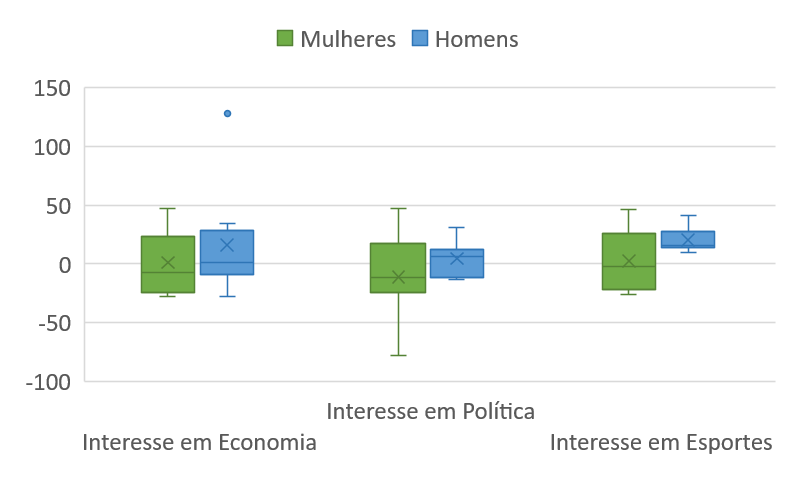
\includegraphics[width=0.6\linewidth]{boxplot_prova_2017_2.png} 
  \caption{Boxplot das preferências por sexo.}
  \label{Fig1}
\end{figure}

(Obs.: o símbolo \(\times\) dentro das caixas indica a média.).

Responda:

\begin{enumerate}
\def\labelenumi{\alph{enumi}.}
\item
  Quais as variáveis analisadas? Classifique-as.
\item
  Utilizando os gráficos de boxplot da figura 1 responda verdadeiro (V)
  ou falso (F):
\end{enumerate}

( \hspace{0,5cm} ) Os respondentes do sexo feminino tiveram preferências
semelhantes entre economia e esportes.

( \hspace{0,5cm} ) No assunto economia, as medianas enre homens e
mulheres são equivalentes.

( \hspace{0,5cm} ) Os homens tenderam a informar um escore de interesse
maior do que as mulheres em todos os assuntos.

( \hspace{0,5cm} ) Os escores no assunto política apresentam
distribuições simétricas.

( \hspace{0,5cm} ) No assunto esporte os escores os escores dos homens
são mais homogêneos do que os escores das mulheres.

\vspace{1.0cm}

\textbf{Questão 4.} Responda verdadeiro (V) se a variável aleatória
presente nos problemas de probabilidade abaixo possui distribuição
binomial ou falso (F) caso contrário:

( \hspace{0,5cm} ) O show 60 minutes do canal de televisão CBS tem sido
um programa de sucesso por muitos anos. Esse show tinha uma audiência de
20, significando que dentro os aparelhos de TV ligados \(20\%\) estavam
sintonizados no 60 Minutes. Suponha que o anunciante deseja verificar se
realmente o valor da audiência é de \(20\%\) realizando a sua própria
pesquisa.

( \hspace{0,5cm} ) Para um período recente de 100 anos, houve 93 grandes
terremotos. Qual a probabilidade de o número de terremotos em um ano ser
igual à 7.

( \hspace{0,5cm} ) Calcule a probabilidade de que o número de clientes
de uma livraria em um dado dia de trabalho seja igual à 40.

( \hspace{0,5cm} ) O tempo médio para realização de determinada tarefa é
de 50 minutos, calcule a probabilidade de que algum indivíduo realize
essa tarefa em menos de 30 minutos.

\newpage

\textbf{Questão 5.} Uma pequena companhia de seguros analisou a
frequência com que todos os seus segurados utilizaram serviços
hospitalares durante um certo período. Os resultados são apresentados na
tabela abaixo.

\begin{center}
\begin{tabular}{cccc}
\hline
  & \multicolumn{2}{c}{Sexo} & \\
\cline{2-3}
Usou serviço hospitalar & Masculino & Feminino & $\sum$ \\ \hline
Sim     & 100 & 150 & 250   \\
Não    & 900 & 850 & 1750  \\ \hline
$\sum$  & 1000 & 1000& 2000  \\ \hline
\end{tabular}
\end{center}

Selecionando-se um segurado ao acaso, responda (utilizando o conceito de
probabilidade frequentista):

\begin{enumerate}
\def\labelenumi{\alph{enumi}.}
\item
  Qual a probabilidade de ser uma mulher e que não tenha utilizado
  serviços hospitalares?
\item
  Qual a probabilidade de ser homem ou tenha utilizado serviços
  hospitalares?
\item
  Sabendo que o segurado é mulher, qual a probabilidade de este ter
  usado serviços hospitalares?
\item
  Qual a probabilidade de ser mulher dado que o segurado não usou
  serviços hospitalares?
\end{enumerate}

\end{document}
